Quantum information with a twist on multiple Hilbert spaces.

\begin{parts}
	\part In general for two Hilbert spaces $\mathcal{H}_1$ and $\mathcal{H}_2$ to be entangled, their composite structure may not be separable.
	
	e.g. for joint density matrix $\rho_\textnormal{AB}$, it cannot decomposed into $\displaystyle \rho_\textnormal{A} \otimes \rho_\textnormal{B} = \sum_{i,\, j} p_i p_j \ket{\psi_i}\bra{\psi_i} \otimes \ket{\psi_j}\bra{\psi_j}$.
	
	\part
	\begin{figure}[H]
		\centering
		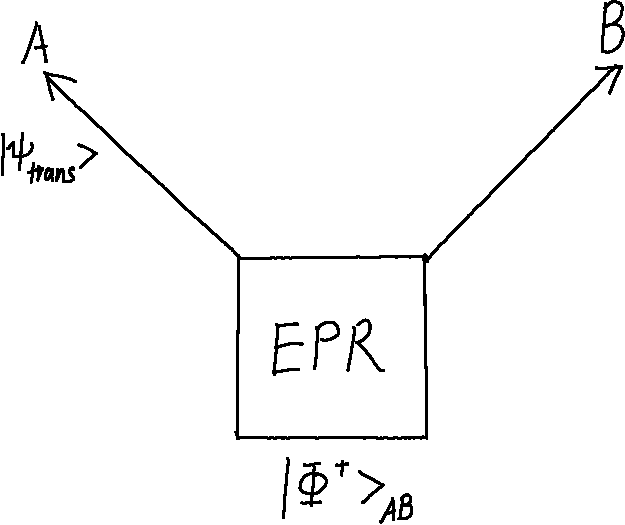
\includegraphics[width=.45\linewidth]{q6-epr}
	\end{figure}
	
	To facilitate quantum teleportation with a Bell state, first the qubit pair has to be distributed between two parties A and B.
	A then performs a Bell state measurement between her qubit with the qubit to be transported $\ket{\psi_\textnormal{trans}} = \alpha\ket{0} + \beta\ket{1}$.
	
	By linearity of Hilbert space, we may rewrite the system state as the superposition of 4 Bell basis \textit{between} $\ket{\psi_\textnormal{trans}}$ and A, and now B has $\ket{\psi_\textnormal{trans}}$ with $\mathds{1}$, X, Y or Z flip.
	Hence if A now communicates the measurement result with B, B may reconstruct $\ket{\psi_\textnormal{trans}}$ without knowing $\ket{\psi_\textnormal{trans}}$ itself!
	
	\part \textit{Here I present a brute-force approach, though a smarter way around this is in my attempt of the 2024 Finals. (Hint: partial trace is your friend)}
	
	\begin{equation*}
		a\ket{00} + b\ket{11} = \begin{pmatrix}
			a \\ 0 \\ 0 \\ b
		\end{pmatrix}
	\end{equation*}
	
	For separable states,
	\begin{equation*}
		\begin{pmatrix}
			\alpha \\ \beta
		\end{pmatrix} \otimes
		\begin{pmatrix}
			\gamma \\ \delta
		\end{pmatrix} =
		\begin{pmatrix}
			\alpha\gamma \\ \alpha\delta \\ \beta\gamma \\ \beta\delta
		\end{pmatrix}
	\end{equation*}
	
	However note that $\alpha\delta = \beta\gamma = 0$ so one of the coefficients in the pairs ($\alpha$, $\beta$) and ($\gamma$, $\delta$) must be 0, which translates to the condition $a=0$ or $b=0$.
	
	\part Suppose instead of $\ket{\Phi^+}$, we have $\ket{\xi} = a\ket{00} + b\ket{11}$ with $a>0$ and $b>0$ and both real.
	The system state may then be described by the following ket vector:
	\begin{align*}
		\ket{\textnormal{sys}} &= \frac{1}{\sqrt{2}} \sbracket{
			\ket{0}_\textnormal{trans} + \ket{1}_\textnormal{trans}
		} \otimes \sbracket{
			a\ket{0_\textnormal{A}0_\textnormal{B}} + b\ket{1_\textnormal{A}1_\textnormal{B}}
		} \\
		&= \frac{1}{\sqrt{2}} \sbracket{
			a\ket{0_\textnormal{trans}0_\textnormal{A}0_\textnormal{B}} + b\ket{0_\textnormal{trans}1_\textnormal{A}1_\textnormal{B}} + a\ket{1_\textnormal{trans}0_\textnormal{A}0_\textnormal{B}} + b\ket{1_\textnormal{trans}1_\textnormal{A}1_\textnormal{B}}
		}
	\end{align*}
	
	We now rewrite:
	\begin{align*}
		\ket{00} = \frac{\ket{\Phi^+} + \ket{\Phi^-}}{\sqrt{2}} & \qquad & \ket{01} = \frac{\ket{\Psi^+} + \ket{\Psi^-}}{\sqrt{2}} \\
		\ket{11} = \frac{\ket{\Phi^+} - \ket{\Phi^-}}{\sqrt{2}} & \qquad & \ket{10} = \frac{\ket{\Psi^+} - \ket{\Psi^-}}{\sqrt{2}}
	\end{align*}
	
	Thus:
	\begin{align*}
		\ket{\textnormal{sys}} &= \frac{1}{\sqrt{2}} \sbracket{
			\frac{a}{\sqrt{2}} \rbracket{
				\ket{\Phi^+}_\textnormal{trans, A}
				+ \ket{\Phi^-}_\textnormal{trans, A}
			}\ket{0_\textnormal{B}} + \frac{b}{\sqrt{2}} \rbracket{
				\ket{\Psi^+}_\textnormal{trans, A}
				+ \ket{\Psi^-}_\textnormal{trans, A}
			}\ket{1_\textnormal{B}}
		+ \right.\\
			&\qquad\left.
			\frac{a}{\sqrt{2}} \rbracket{
				\ket{\Psi^+}_\textnormal{trans, A}
				- \ket{\Psi^-}_\textnormal{trans, A}
			}\ket{0_\textnormal{B}} + \frac{b}{\sqrt{2}} \rbracket{
				\ket{\Phi^+}_\textnormal{trans, A}
				- \ket{\Phi^-}_\textnormal{trans, A}
			}\ket{1_\textnormal{B}}} \\
		&= \frac{1}{2} \sbracket{
			\ket{\Phi^+}_\textnormal{trans, A} \rbracket{
				a\ket{0_\textnormal{B}}
				+ b\ket{1_\textnormal{B}}
			} + \ket{\Phi^-}_\textnormal{trans, A} \rbracket{
				a\ket{0_\textnormal{B}}
				- b\ket{1_\textnormal{B}}
			} + \right.\\
		&\qquad\left.
			\ket{\Psi^+}_\textnormal{trans, A} \rbracket{
				a\ket{0_\textnormal{B}}
				+ b\ket{1_\textnormal{B}}
			} + \ket{\Psi^-}_\textnormal{trans, A} \rbracket{
				-a\ket{0_\textnormal{B}}
				+ b\ket{1_\textnormal{B}}
			}
		}
	\end{align*}
	
	Note that the amplitudes $a$ and $b$ are carried over due to the linearity of Hilbert space, thus the fidelity of the output state is:
	\begin{align*}
		\mathcal{F} &= \abs{\rbracket{a\bra{0} + b\bra{1}} \rbracket{\frac{1}{\sqrt{2}}\ket{0} + \frac{1}{\sqrt{2}}\ket{1}}}^2 \\
		&= \abs{\frac{a}{\sqrt{2}} + \frac{b}{\sqrt{2}}}^2 \\
		&= \frac{a^2 + b^2}{2} + ab \\
		&= \frac{1}{2} + ab
	\end{align*}
	
	\part Now suppose $\ket{\psi_\textnormal{trans}}$ is entangled to some other system, so $\ket{\psi_\textnormal{trans}} = \alpha\ket{0} \otimes \rho_0 + \beta\ket{1} \otimes \rho_1$ where $\rho_{0,\, 1}$ are the entangled external entities.
	
	Repeating the scheme above and it is clear that $\rho_0$ always follow the coefficient $\alpha$ and $\rho_1$ with $\beta$, so after the transportation, we realise that $\ket{\psi_\textnormal{B}} = \ket{\psi_\textnormal{trans}}$ \textit{precisely}, hence the entanglement is also transported.
\end{parts}